\subsection{Risultati sperimentali}
\label{sec:results}
Proponiamo alcuni risultati sperimentali ottenuti dal package Python contenente gli algoritmi per il calcolo della massima bisimulazione che abbiamo presentato nelle sezioni precedenti. Innanzitutto illustreremo brevemente l'ambiente e gli strumenti con cui sono state prese le misurazioni. Dopodichè presenteremo i risultati in forma di grafici, e tenteremo di evidenziare le differenze tra i vari algoritmi.

\subsubsection{Hardware e strumenti per le misura}
I risultati sono stati misurati su un computer con sistema operativo \emph{CentOS Linux}, architettura x86\_64, processore \emph{Intel(R) Core(TM) i7-4790 CPU} (4 cores, 3.60GHz), e memoria RAM da 16 GB. Per ottenere le misurazioni è stato utilizzato il package Python \emph{timeit}, che presenta alcune caratteristiche che lo rendono un valido strumento per la misurazione del tempo di esecuzione \cite{pythondocs}:
\begin{itemize}
    \item Utilizza la più precisa funzione disponibile sulla piattaforma per la misurazione del tempo trascorso;
    \item Disabilita il \emph{garbage collector}, che potrebbe intervenire in un momento casuale della misurazione introducendo rumore nei risultati;
    \item Esegue lo script preso in esame molte volte in modo da ridurre l'imprecisione dovuta a temporanei sovraccarichi della CPU o della RAM.
\end{itemize}

I dataset su cui abbiamo effettuato le misurazioni sono stati generati utilizzando alcune funzioni del package Python \emph{NetworkX} \cite{networkx}.

\subsubsection{Performance}
Consideriamo alcune tipologie differenti di grafi, e valutiamo il tempo necessario per l'esecuzione degli algoritmi che abbiamo implementato. Nei grafici utilizziamo lungo l'asse delle ascisse una scala data dal valore $|E| \log |V|$, che ci consente di visualizzare in modo più omogeneo i risultati lungo l'asse delle ordinate. Entrambi gli assi variano secondo una scala logaritmica.

\paragraph{Paige-Tarjan, Dovier-Piazza-Policriti} Cominciamo confrontando gli algoritmi di Paige-Tarjan e Dovier-Piazza-Policriti: ci aspettiamo che quest'ultimo risulti asintoticamente più conveniente. Per grafi piccoli invece dovrebbe risultare vincitore l'algoritmo di Paige-Tarjan visto che non richiede l'elaborazione preliminare del rango.

Cominciamo l'esposizione dei risultati con la categoria degli ``alberi bilanciati'', ovvero grafi che possono essere rappresentati nella forma esposta nella Figura \ref{fig:balanced_tree}. Essi sono caratterizzati da due parametri:
\begin{itemize}
    \item \emph{depth}: il numero di livelli (senza contare la \emph{root});
    \item \emph{branching factor}: il numero di successori di ogni nodo (ad eccezione dei nodi nell'ultimo livello).
\end{itemize}

Generiamo grafi di questo tipo tramite la funzione \verb|balanced_tree| di \emph{NetworkX}, che appunto prende in input questi due parametri.

\begin{figure}
    \centering
    \begin{subfigure}[b]{0.4\textwidth}
        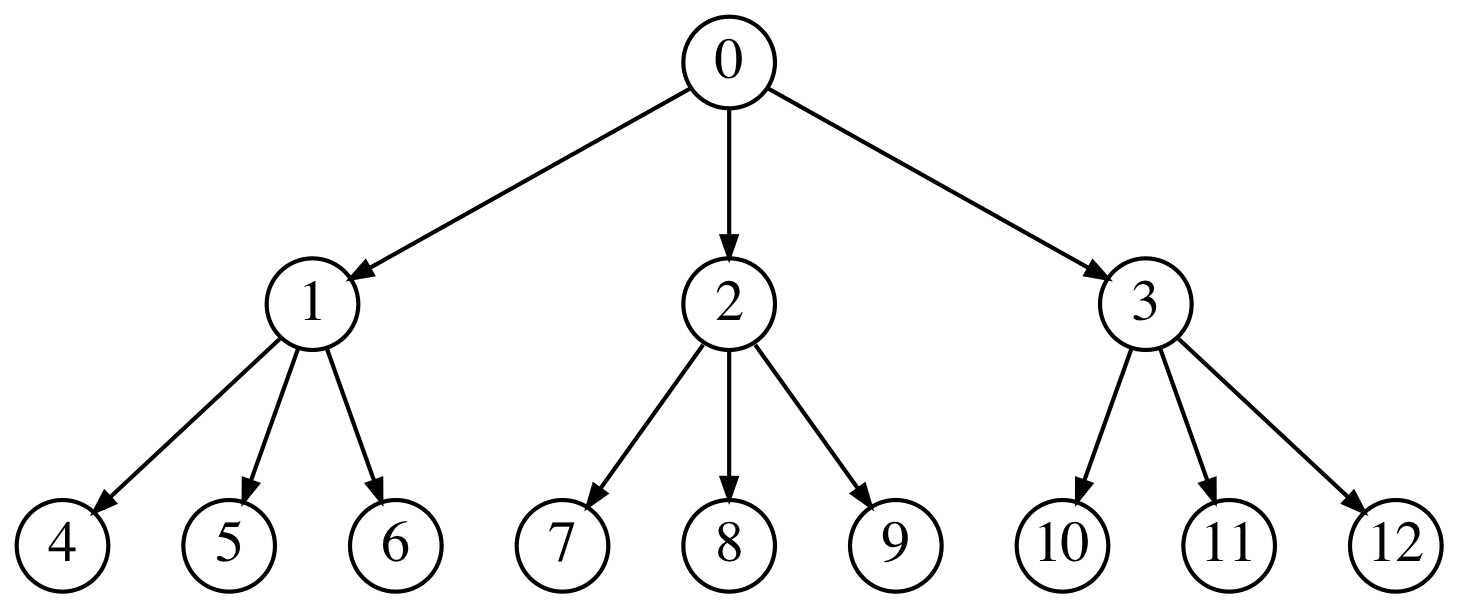
\includegraphics[width=\textwidth]{./sezione3/experimental_results/plots/tree_graph.png}
        \caption{Un albero bilanciato, \emph{depth}=2, \emph{branching factor}=3.}
        \label{fig:balanced_tree}
    \end{subfigure}
    \qquad
    \begin{subfigure}[b]{0.1\textwidth}
        \centering
        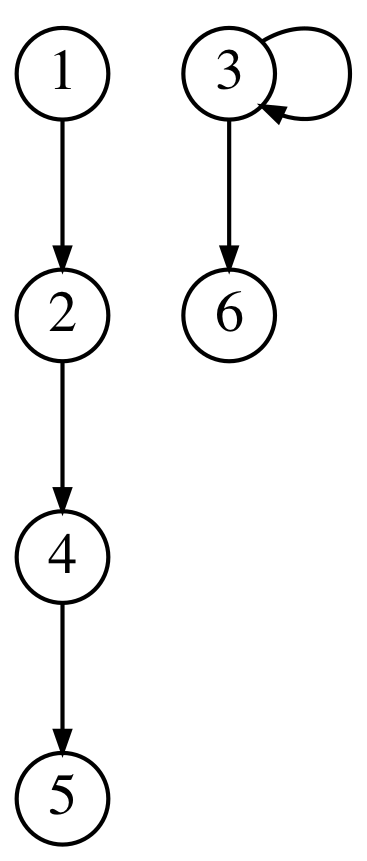
\includegraphics[width=\textwidth]{./sezione3/experimental_results/plots/hopcroft_graph_1.png}
        \caption{Hopcroft, $n=2$}
        \label{fig:hopcroft_graph_1}
    \end{subfigure}
    \qquad \qquad
    \begin{subfigure}[b]{0.2\textwidth}
        \centering
        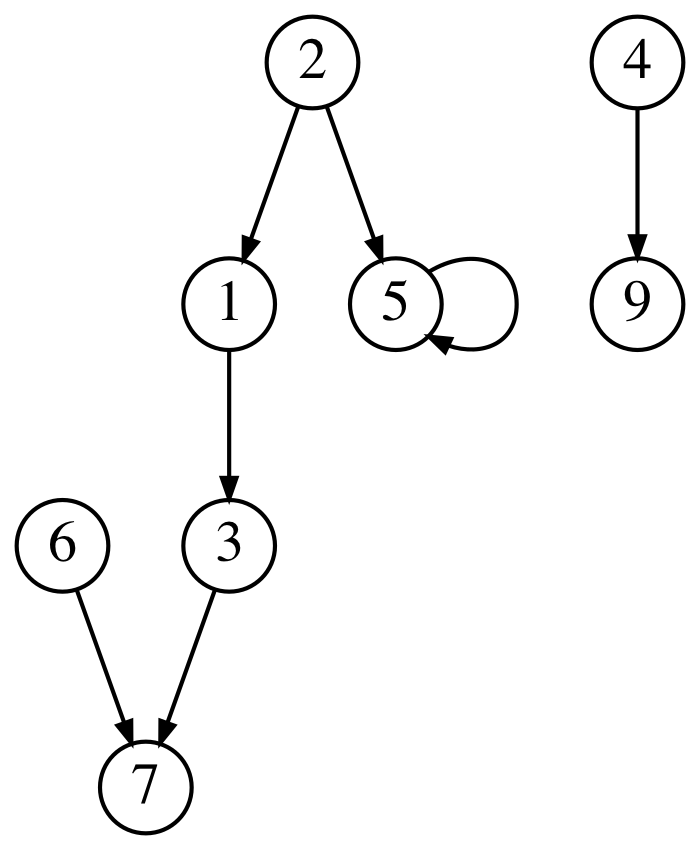
\includegraphics[width=\textwidth]{./sezione3/experimental_results/plots/hopcroft_graph_2.png}
        \caption{Hopcroft, $n=3$}
        \label{fig:hopcroft_graph_2}
    \end{subfigure}
    \caption{Tipologie di grafi su cui abbiamo testato gli algoritmi di Dovier-Piazza-Policriti e Paige-Tarjan.}
\end{figure}

\begin{figure}[b!]
    \begin{subfigure}[t]{0.5\textwidth}
        \begin{tikzpicture}
            \begin{axis}[
                axis on top,
                width=\textwidth,
                ytick style={draw=none},
                xtick style={draw=none},
                xmode=log,
                ymode=log,
                grid=major
            ]
            \addplot table[x=x,y=y] {experiments/time/tree/pta.txt};
            \label{fig:pta_line_tree}
            \addplot table[x=x,y=y] {experiments/time/tree/fba.txt};
            \label{fig:fba_line_tree}
            \end{axis}
        \end{tikzpicture}
        \caption{Alberi bilanciati con \emph{depth} e \emph{branching factor} variabili.}
        \label{fig:tree_exp_result}
    \end{subfigure}
    \begin{subfigure}[t]{0.5\textwidth}
        \begin{tikzpicture}
            \begin{axis}[
                axis on top,
                width=\textwidth,
                ytick style={draw=none},
                xtick style={draw=none},
                grid=major,
                xmode=log,
                ymode=log
            ]
            \addplot table[x=x,y=y] {experiments/time/hopcroft/pta.txt};
            \label{fig:pta_line_hopcroft}
            \addplot table[x=x,y=y] {experiments/time/hopcroft/fba.txt};
            \label{fig:fba_line_hopcroft}
            \end{axis}
        \end{tikzpicture}
        \caption{Grafi della tipologia elaborata da Hopcroft, di dimensioni varie.}
        \label{fig:hopcroft_exp_result}
    \end{subfigure}
    \caption{Tempo di esecuzione degli algoritmi di Dovier-Piazza-Policriti (\ref*{fig:fba_line_tree}) e Paige-Tarjan (\ref*{fig:pta_line_tree}) sulle tipologie di grafo \ref{fig:balanced_tree} (a) e \ref{fig:hopcroft_graph_1}, \ref{fig:hopcroft_graph_2} (b). Lungo l'asse delle ascisse (logaritmico) abbiamo la quantità $|E|\log|V|$, mentre sull'asse delle ordinate (logaritmico) è riportato il tempo di esecuzione dell'algoritmo in secondi.}
\end{figure}

Dalla Figura \ref{fig:tree_exp_result} possiamo osservare che asintoticamente l'algoritmo di Dovier-Piazza-Policriti è asintoticamente più efficiente, a partire da un certo valore di $|E| \log |V|$. Sebbene infatti la metodologia sia più ``rifinita'' dell'approccio di Paige-Tarjan, lo sforzo iniziale per il calcolo del rango è apprezzabile, soprattutto se consideriamo il linguaggio in cui l'algoritmo è stato implementato. Abbiamo però la conferma che per valori alti di $|E| \log |V|$, per questa tipologia di grafo, si ottengono i risultati previsti.

La seconda tiplogia di grafi che consideriamo è tratta dall'articolo in cui viene presentato l'algoritmo di Dovier-Piazza-Policriti, ed è un esempio di automa proposto originariamente da Hopcroft \cite{hopcroft}. Nelle Figure \ref{fig:hopcroft_graph_1} e \ref{fig:hopcroft_graph_2} ne visualizziamo alcune realizzazioni.

In Figura \ref{fig:hopcroft_exp_result} sono riportati i risultati ottenuti dagli algoritmi. Osserviamo nuovamente che l'algoritmo di Dovier-Piazza-Policriti risulta asintoticamente più conveniente anche in questo caso.

\paragraph{Dovier-Piazza-Policriti, Saha} Proseguiamo l'esposizione dei risultati sperimentali ottenuti utilizzando il pacchetto \texttt{BisPy} con un confronto tra gli algoritmi di Dovier-Piazza-Policriti (Sezione \ref{sec:dovier_piazza_policriti}) e l'algoritmo incrementale di Saha (Sezione \ref{sec:saha}). L'obiettivo di questo confronto è verificare che l'algoritmo incrementale risulti più efficiente nel ricalcolare la massima bisimulazione in seguito all'aggiunta di un nuovo arco, rispetto ad un algoritmo che non sfrutti le informazioni relative alla massima bisimulazione prima della modifica. Rammentiamo la complessità dell'algoritmo incrementale, calcolata nella Sezione \ref{sec:saha_complexity}:
\begin{align*}
    T_{\text{Saha}} = O(|E_1|\log|V_1|) &+ O(|\Delta_{\wf}\log|\Delta_{\wf}|) + O(|E_{\nwf}| + |V_{\nwf}|)\\
    &+ O(|E_2||V_2|) + O(|E_2|\log|V_2|)
\end{align*}
$\Delta_\nwf$ è l'insieme di nodi \emph{non-well-founded} il cui rango è cambiato in seguito all'inserimento del nuovo arco; $E_1,V_1$ e $E_2,V_2$ sono rispettivamente nodi e archi appartenenti al sottografo di $G$ composto dai nodi modificati durante le fasi 1. (\funcname{split}) e 2. (\funcname{merge}); $E_{\nwf}$, $V_{\nwf}$ sono rispettivamente archi e nodi del sottografo \emph{non-well-founded} di $G$.

Si osservi che numerosi termini possono diventare molto facilmente ``problematici'', e rendere quindi l'algoritmo incrementale meno efficiente del ricalcolo da zero della massima bisimulazione. In questa breve analisi presenteremo i risultati su alcune tipologie di grafo, e ne verificheremo la coerenza con l'analisi proposta nelle sezioni precedenti.

\subsubsection{Dimensione della massima bisimulazione}
Terminiamo la sezione relativa ai risultati sperimentali con un'ultima analisi che potrebbe essere di qualche interesse nella prospettiva di ciò che abbiamo presentato nella Sezione \ref{sec:applications}. Consideriamo l'andamento del numero di classi di equivalenza nella massima bisimulazione per grafi di Erdős-Rényi (o \emph{grafi binomiali}), ovvero grafi contenenti un numero arbitrario \verb|n| di nodi, per cui presa una coppia qualsiasi $u,v \in V$ si ha $\langle u,v\rangle \in E$ con probabilità \verb|p| $< 1$.
Considereremo valori piccoli di \verb|p|, in quanto avvicinandoci ad 1 otteniamo grafi sempre più ``completi'' di interesse molto basso nella pratica. Nella Figura \ref{fig:bisi_size} abbiamo considerato tre diversi valori per il parametro \verb|n|, e quattro valori per il parametro \verb|p|.

\begin{figure}[H]
    \begin{center}
        \begin{subfigure}[b]{0.3\textwidth}
            \begin{tikzpicture}[scale=1.3]
                \begin{axis}[
                    axis on top,
                    width=\textwidth,
                    legend columns=-1,
                    legend style={/tikz/every even column/.append style={column sep=0.5cm}},
                    legend entries={$p=0.01$, $p=0.05$, $p=0.1$, $p=0.2$},
                    legend to name=named,
                    tick pos=both,
                    xtick style={color=black},
                    ytick style={color=black},
                    grid=both,
                    title={$n=10$}
                ]
                \addplot[scatter, scatter/classes={
                    a={mark=asterisk,blue},
                    b={mark=diamond,red},
                    c={mark=square,green},
                    d={mark=triangle,yellow}
                    }, only marks, scatter src=explicit symbolic] table[y=y,meta=label] {experiments/dimension/dim/result10.txt};
                \end{axis}
            \end{tikzpicture}
        \end{subfigure}
        \begin{subfigure}[b]{0.3\textwidth}
            \begin{tikzpicture}[scale=1.3]
                \begin{axis}[
                    axis on top,
                    width=\textwidth,
                    tick pos=both,
                    xtick style={color=black},
                    ytick style={color=black},
                    grid=both,
                    title={$n=100$}
                ]
                \addplot[scatter, scatter/classes={
                    a={mark=asterisk,blue},
                    b={mark=diamond,red},
                    c={mark=square,green},
                    d={mark=triangle,yellow}
                    }, only marks, scatter src=explicit symbolic] table[y=y,meta=label] {experiments/dimension/dim/result100.txt};
                \end{axis}
            \end{tikzpicture}
        \end{subfigure}
        \begin{subfigure}[b]{0.3\textwidth}
            \begin{tikzpicture}[scale=1.3]
                \begin{axis}[
                    axis on top,
                    width=\textwidth,
                    tick pos=both,
                    xtick style={color=black},
                    ytick style={color=black},
                    grid=both,
                    title={$n=1000$}
                ]
                \addplot[scatter, scatter/classes={
                    a={mark=asterisk,blue},
                    b={mark=diamond,red},
                    c={mark=square,green},
                    d={mark=triangle,purple}
                    }, only marks, scatter src=explicit symbolic] table[y=y,meta=label] {experiments/dimension/dim/result1000.txt};
                    \label[a]{fig:bisi_size_1000_p001}
                    \label[b]{fig:bisi_size_1000_p005}
                    \label[c]{fig:bisi_size_1000_p01}
                    \label[d]{fig:bisi_size_1000_p02}
                \end{axis}
            \end{tikzpicture}
        \end{subfigure}
        \ref*{named}
    \end{center}
    \caption{Numero di classi di equivalenza della massima bisimulazione per grafi generati in modo casuale, normalizzato rispetto al numero di nodi nel grafo. Ad ogni \emph{tick} sull'asse delle ascisse corrisponde un grafo generato in modo casuale. Lungo l'asse delle ordinate è riportato il numero di blocchi della bisimulazione massima.}
    \label{fig:bisi_size}
\end{figure}

Per ogni combinazione di \verb|n|,\verb|p| abbiamo generato 100 grafi binomiali con la funzione \verb|fast_gnp_random_graph| del pacchetto \emph{NetworkX}, e ne abbiamo calcolata la massima bisimulazione con l'algoritmo di \emph{Dovier-Piazza-Policriti}. Nei grafici abbiamo visualizzato la quantità $\frac{|V / \equiv|}{|V|}$, ovvero il rapporto tra il numero di classi di equivalenza nella massima bisimulazione ed il numero di nodi del grafo: questa quantità potrebbe essere considerata come il fattore di riduzione che otteniamo quanto sostuitiamo al grafo originale la sua contrazione secondo la massima bisimulazione.

Per \verb|n=10| la quantità che stiamo valutando varia molto tra 1 (10 classi di equivalenza, nessuna riduzione) e 0.1 (tutti i nodi sono bisimili, riduzione massima). Per valori più grandi la variabilità si riduce, e per \verb|n=1000| il fattore si schiaccia decisamente verso 0.001 (un'unica partizione).
